\documentclass[a4paper,11pt]{article}
\usepackage[framed,numbered]{matlab-prettifier}
\usepackage{caption}
\usepackage{graphicx}
\usepackage{subcaption}
\begin{document}
	\begin{titlepage}
		
		\newcommand{\HRule}{\rule{\linewidth}{0.5mm}} % Defines a new command for the horizontal lines, change thickness here
		
		\center % Center everything on the page
		
		
		
		\textsc{\LARGE Department of  }\\[0.3cm] % Name of your university/college
		\textsc{\LARGE Robotics and Mechatronics Engineering  }\\[0.3cm]
		\textsc{\Large   }\\[0.3cm]
		\textsc{\Large Lab report }\\[0.5cm] % Major heading such as 
		
		\HRule \\[0.4cm]
		{ \huge \bfseries DIGITAL SIGNAL PROCESSING}\\[0.4cm]  
		
		{ \huge \bfseries (CSE-401)}\\[0.03cm]
		% Title of your document
		
		\HRule 
		\\
		\large{\bfseries{Name of the Experiment:} Filter design in frequency domain.}
		\\[5cm]
		
		
		
		\begin{minipage}{0.4\textwidth}
			\begin{flushleft} \large
				\emph{Submitted By:}\\
				Md. Tahmeed Abdullah \\Roll: SH-092-002\\$4^{th}$ year $1^{st}$ semester % Your name
			\end{flushleft}
		\end{minipage}
		~
		\begin{minipage}{0.4\textwidth}
			\begin{flushright} \large
				\emph{Submitted To:} \\
				Mr. Sujan Sarker\\Lecturer\\Dept. of RME % Supervisor's Name
			\end{flushright}
		\end{minipage}\\[1cm]
		
		
		
		\vfill
			
		
		
	\end{titlepage}
	\begin{center}
		
	\end{center}
	\section*{Experiment no. 6}
	\section*{Name of the experiment}
	Filter design in frequency domain.
	\section*{Objectives}
	\begin{itemize}
		\item To learn how to use filters. 
		\item To understand the concepts of High pass filter and Low Pass filter.
		\item To learn to design filters using cutoff frequency.
		\item To sharpen or blur an image using filters in frequency domain.
		
	\end{itemize}
	\section*{Theory}
	Fast Fourier Transform maps a two dimensional image from spatial domain to the frequency domain. As a result we obtain a matrix of complex numbers. 
	
	A window of circular shape of radius equal to the cutoff frequency can cut off the frequency components outside the circle. Thus this window acts as a \emph{Low Pass Filter}. If this filtered frequency components are again mapped to spatial domain using Inverse Fast Fourier Transform we get a an image which is blurred out. The frequency of pixel values are higher at the edges. So, the edges are smoothed and thus we get a blurred image.
	
	Again, if a window is taken which allows frequency components outside a circle of radius equal to cutoff frequency we get higher frequency values only. If the filtered frequency components are mapped to spatial domain using Inverse Fourier Transform we get only the edges of the images. The threshold of edge remaining can be controlled by the radius of the circle of the filter i.e. by changing the cut-off frequency. Thus, in such a manner \emph{High Pass Frequency} is actualized.
	
	
	\section*{Implementation Code}  
	\captionsetup{labelformat=empty,labelsep=none}
	\lstinputlisting[style = Matlab-editor,frame=bt, caption={main.m}]{../lab6.m}
	\vspace*{8.7cm}
	\section*{Result}
	\begin{figure}[h!]
		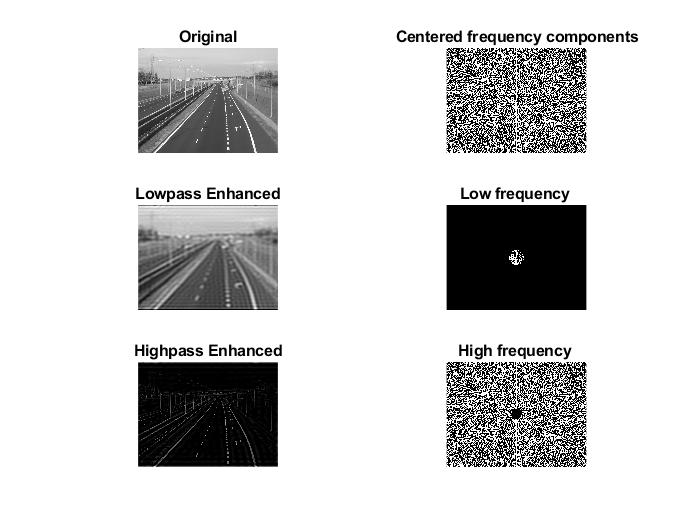
\includegraphics[scale=0.6]{result.jpg}
		\caption{High Pass Filter and Low Pass Filter Visualized}
	\end{figure}  
	
\end{document}